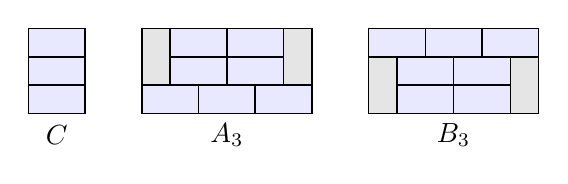
\begin{tikzpicture}[x=0.36cm,y=0.36cm,line width=0.55pt]
\begin{scope}
 \foreach \y in {0,1,2}{\draw[fill=blue!9] (0,\y) rectangle ++(2,1);}
 \node at (1,-0.75) {$C$};
\end{scope}
\begin{scope}[shift={(4,0)}]
 \draw[fill=gray!20] (0,1) rectangle (1,3);
 \draw[fill=gray!20] (5,1) rectangle (6,3);
 \foreach \x in {0,2,4}{\draw[fill=blue!9] (\x,0) rectangle ++(2,1);}
 \foreach \y in {1,2}{\foreach \x in {1,3}{\draw[fill=blue!9] (\x,\y) rectangle ++(2,1);}}
 \node at (3,-0.75) {$A_3$};
\end{scope}
\begin{scope}[shift={(12,0)}]
 \draw[fill=gray!20] (0,0) rectangle (1,2);
 \draw[fill=gray!20] (5,0) rectangle (6,2);
 \foreach \x in {0,2,4}{\draw[fill=blue!9] (\x,2) rectangle ++(2,1);}
 \foreach \y in {0,1}{\foreach \x in {1,3}{\draw[fill=blue!9] (\x,\y) rectangle ++(2,1);}}
 \node at (3,-0.75) {$B_3$};
\end{scope}
\end{tikzpicture}
